There are two ways two play the game, either by deploying the game to the Xbox 360 and play it on the console, or 
run the game on Windows with two Xbox 360 controllers attached. We have written a manual for both, so the reader can 
test the game according to his/her preferences. 

\subsection{Xbox 360}

In order to play the game on the Xbox 360 Console, there are several prerequisites to take into account. Firstly, 
the following is mandatory\cite{deploy}:

\begin{itemize}
	\item Computer running Windows with XNA Game Studio 4.0 
	\item Xbox 360 Console with two controllers
	\item XNA Game Studio Connect on the Xbox 360 Console 
	%\item Atleast an Silver Xbox LIVE membership \\
	%\item XNA Creators Club premium membership \\
	\item Hard drive on the Xbox 360 to deploy the game onto 
\end{itemize}

\subsubsection{Connecting the Xbox 360 Console with XNA Game Studio 4.0}

Note! In order to download \textbf{XNA Game Studio Connect}, the Xbox 360 console needs an internet connection. \\

\begin{enumerate}
	\item On the Xbox 360 Console, navigate to \textbf{Game Marketplace}.
	\item Select \textbf{Explore Game Content} and then \textbf{Browse}. 
	\item When your at the \textbf{All Games} screen browse to \textbf{Genre} and select \textbf{Other}. 
	\item Scroll to \textbf{XNA Creators Club} and select it. 
	\item From this pane, select \textbf{All Downloads}, then select \textbf{XNA Game Studio Connect}. 
	\item \textbf{Confirm Download} to begin downloading. 
\end{enumerate}

In order to deploy the game to the Xbox 360 console, the development computer and the Xbox 360 needs to be on the same subnet on the local network. If the computer and console is behind the same router, it is very likely that you're on the same subnet. In order to deploy the game a \textbf{connection key} needs to be generated. \\

\begin{enumerate}
	\item On the Xbox 360 Console, go to \textbf{My Xbox} and select \textbf{Game Library}. 
	\item then go to \textbf{Collections} tab and select \textbf{Community Games}. 
	\item Select \textbf{XNA Game Studio Connect} and then select \textbf{Launch}. 
	\item The XNA Game Studio connect screen will appear: \\ \begin{center}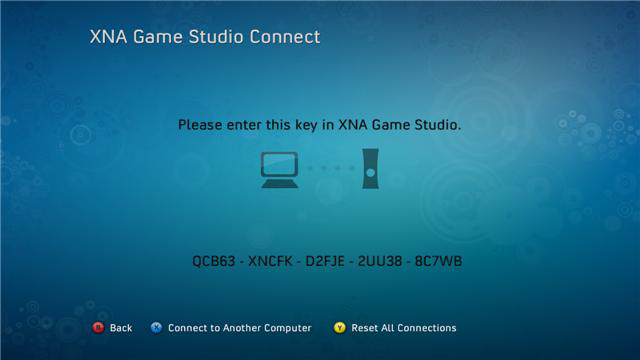
\includegraphics[scale=0.5]{graphics/connect}\end{center}
	\item If a \textbf{Connection Key} is displayed go to step \ref{generated}. 
	\item If the \textbf{Connection Key} does not appear, the Xbox 360 console could already be connected to this computer. The game studio supports multiple connection keys for multiple computers. To add a new connection press \textbf{X}. 
	\item \label{generated} On your computer, go to the \textbf{Start} menu, select \textbf{programs} and then select \textbf{XNA Game Studio 4.0}. 
	\item Launch the \textbf{XNA Game Studio Device Center}.
	\item Click \textbf{Add Device} \\ \begin{center}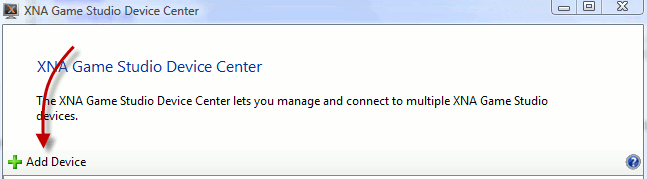
\includegraphics[scale=0.75]{graphics/add_device}\end{center} 
	\item Select the type type of device to be \textbf{Xbox 360} \\ \begin{center}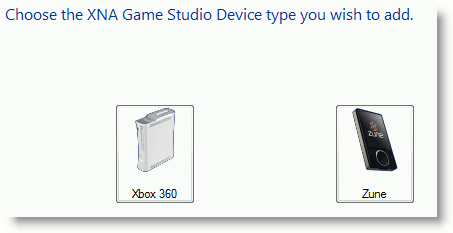
\includegraphics[scale=0.75]{graphics/type_of_device}\end{center} 
	\item Enter a name for the console and press \textbf{Next}. 
	\item Enter the connection key that is displayed in the XNA Game Studio Connect on the Xbox 360 console. 
	\item Once you have typed in the correct key, press \textbf{Next} on the \textbf{XNA Game Studio Devices} dialog box. 
	\item The XNA Game Studio Device center will test the connection. If it fails, pay attention to the error message of the dialog box. If it did not result from a mismatched key, please refer to \cite{troubleshoot}. 
	\item Click \textbf{Finish}. The console will now be listed in the XNA Game Studio Device Center  
\end{enumerate}

\subsubsection{Deploying the game to Xbox360}

\begin{enumerate}	
	\item On the development computer, fire up the project in Visual Studio.
	\item Then go to the Xbox 360 console and go to \textbf{My Xbox} and then select \textbf{Game Library}. 
	\item From \textbf{Game Library}, go to the \textbf{Collections} tab and then select \textbf{Community Games}
	\item Select \textbf{XNA Game Studio Connect} and then select Launch, which will display a screen like this: \\ \begin{center}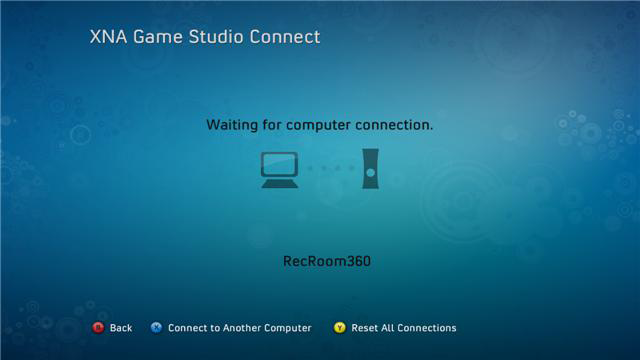
\includegraphics[scale=0.5]{graphics/connect2}\end{center}
	\item On your computer, build the project, deploy the needed files Xbox 360 and then run.
	\item Now you have deployed the game. 
	\item The game will appear in \textbf{Recent games} in the \textbf{Game Library}.	 
\end{enumerate}

\subsection{Playing the game on a (Windows) computer}

In order to play the game on a Windows computer, you need at least two Xbox 360 controllers. To connect a controller to the PC, you will need a USB cable connector from the controller to the computer. From this point, simply execute the executable file, and play! 


